\chapter{Heaps and Heapsort}

\section{Introduction to Heaps}
\begin{figure}[h!]
    \centering
    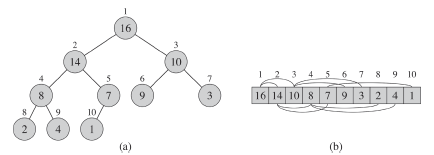
\includegraphics[width=0.75\linewidth]{immagini/heap1.png}
\end{figure}
Heaps are a foundational data structure in computer science used for efficient sorting and priority management. They offer:
\begin{itemize}
    \item Sorting algorithm with \( O(n \log n) \) complexity.
    \item An in-place sorting mechanism.
    \item A design that uses a specific data structure to manage information during execution.
    \item Applications in sorting (\textit{Heapsort}) and other efficient structures like priority queues.
\end{itemize}

\section{The Heap Data Structure}
A \textbf{heap} is an array-based data structure often represented as a nearly complete binary tree:
\begin{itemize}
    \item The tree is filled level by level, with the last level filled from left to right. The first element will always be the root.
    \item An array \( A \) representing a heap has attributes:
    \begin{itemize}
        \item \texttt{length[A]}: Total size of the array.
        \item \texttt{heap-size[A]}: Number of elements in the heap, with \( \texttt{heap-size[A]} \leq \texttt{length[A]} \).
    \end{itemize}
\end{itemize}
\begin{figure}[H]
    \centering
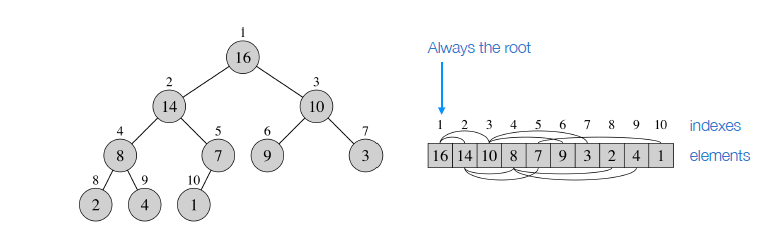
\includegraphics[width=0.8\linewidth]{Heap structure.png}
    \caption{}
    \label{fig:enter-label}
\end{figure}


\subsection{Heap Properties}
\begin{itemize}
    \item The root is stored at \( A[1] \).
    \item For an element at index \( i \):
    \begin{itemize}
        \item Parent: \( A[\lfloor i/2 \rfloor] \).
        \item Left child: \( A[2i] \).
        \item Right child: \( A[2i+1] \).
    \end{itemize}
    \item \textbf{Max-heap property:} \( A[\text{parent}(i)] \geq A[i] \).
    \item \textbf{Min-heap property:} \( A[\text{parent}(i)] \leq A[i] \).
\end{itemize}
\subsection{exercise}
\begin{figure}[h!]
    \centering
    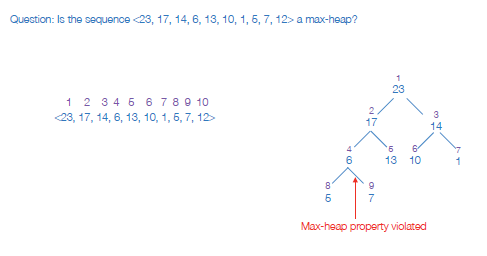
\includegraphics[width=1\linewidth]{immagini/heap2.png}
\end{figure}

\begin{figure}[H]
    \centering
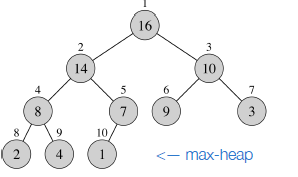
\includegraphics[width=0.5\linewidth]{heap prop.png}
    \label{fig:enter-label}
\end{figure}


\section{Max-Heapify}
The \textbf{Max-Heapify} operation ensures the max-heap property by adjusting the heap from a specific index downward.

\subsection{Algorithm: Max-Heapify}
\begin{verbatim}
MAX-HEAPIFY(A, i)
l = left(i)
r = right(i)
if l <= heap-size[A] and A[l] > A[i] then
    largest = l
else
    largest = i
if r <= heap-size[A] and A[r] > A[largest] then
    largest = r
if largest != i then
    exchange A[i] with A[largest]
    MAX-HEAPIFY(A, largest)
\end{verbatim}

\textbf{Complexity:} \( O(\log n) \), proportional to the height of the tree.
\begin{figure}[h!]
    \centering
    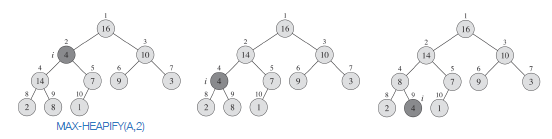
\includegraphics[width=1\linewidth]{immagini/heap3.png}
\end{figure}
\section{Building a Max-Heap}
\textbf{BUILD-MAX-HEAP} constructs a max-heap from an unordered array.

\subsection{Algorithm: Build-Max-Heap}
\begin{verbatim}
BUILD-MAX-HEAP(A)
heap-size[A] = length[A]
for i = floor(length[A]/2) downto 1 do
    MAX-HEAPIFY(A, i)
\end{verbatim}
\textbf{Complexity:} \( O(n) \). This is more efficient than the naive \( O(n \log n) \) bound because most heap levels have fewer nodes. \newline
\textbf{How does it work?} The algorithm starts checking from the element $\lfloor len(A)/2 \rfloor$ and then works its way back up. In each step, it fixes everything before moving on. Note that the system always looks down and not up, using \textbf{MAX-HEAPIFY(A,1)} we always consider the first element that looks at the entire graph.
\subsection{Exercise}
    \begin{figure}[h!]
        \centering
        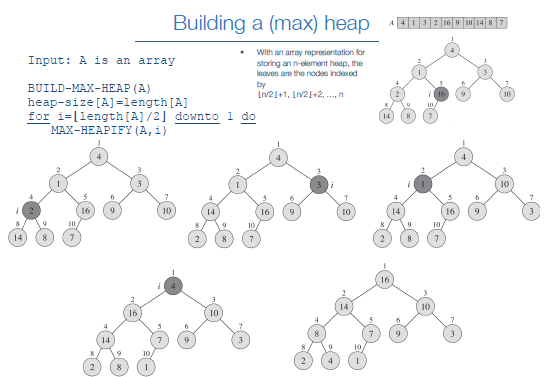
\includegraphics[width=1\linewidth]{immagini/heap4.png}
    \end{figure}
The loop could not go from 1 to floor(length[A]/2) because it could not guarantee the maxheap property. E.g. A [2,1,1,3] then MAX-HEAPIFY won’t exchange 2 with it’s children (1’s). However, when MAX-HEAPIFY is called on the left child, 1, it will swap 1 with 3. This violates the max-heap property because now 2 is the parent of 3. An upper bound of the running time is O(n log n) because MAX-HEAPIFY costs O(log n) and we call it O(n) times. It is possible to derive a tighter upper bound by observing that the time required by MAXHEAPIFY varies with the height of the node and most heights are small. It can be proved that BUILD-MAX-HEAP run in O(n).
    
\section{Heapsort}
\textbf{Heapsort} is a sorting algorithm that uses a heap to organize data efficiently.

\subsection{Algorithm: Heapsort}
\begin{verbatim}
HEAPSORT(A)
BUILD-MAX-HEAP(A) #O(n)
for i = len(A) downto 2 do #O(n-1)
    exchange A[1] with A[i] #O(1)
    A.heap-size = A.heap-size - 1 #O(1)
    MAX-HEAPIFY(A, 1) #O(logn)
\end{verbatim}
\textbf{Complexity:} \( O(n) + O((n-1)(\log n)) = O(n \log n) \).

\subsection{Exercise 1}
    \begin{figure}[h!]
        \centering
        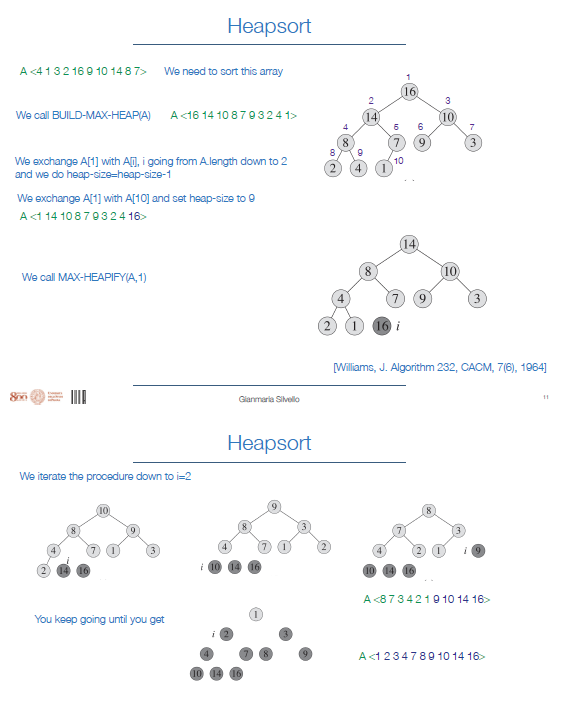
\includegraphics[width=1\linewidth]{immagini/heap5.png}
    \end{figure}
\newpage
\subsection{Exercise 2}
    \begin{figure}[h!]
        \centering
        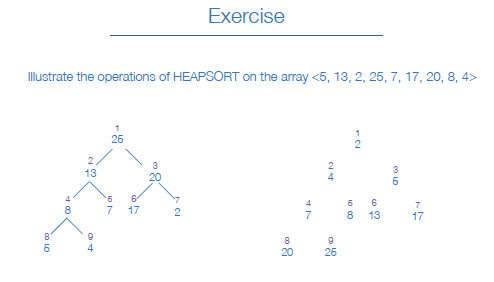
\includegraphics[width=0.8\linewidth]{immagini/heap6.png}
    \end{figure}

\section{Priority Queues}
Priority queues are abstract data structures for managing elements with associated priorities.

\subsection{Operations}
\begin{itemize}
    \item \texttt{INSERT(S, x)}: Add element \( x \) to \( S \).
    \item \texttt{MAXIMUM(S)}: Return the element with the maximum key.
    \item \texttt{EXTRACT-MAX(S)}: Remove and return the element with the maximum key.
    \item \texttt{INCREASE-KEY(S, x, k)}: Increase the key of \( x \) to \( k \) (\( k \geq \) current key).
\end{itemize}

\subsection{Complexity}
If implemented with a heap:
\begin{itemize}
    \item \texttt{INSERT(S, x)}: \( O(\log n) \).
    \item \texttt{MAXIMUM(S)}: \( O(1) \).
    \item \texttt{EXTRACT-MAX(S)}: \( O(\log n) \).
\end{itemize}